\section{The algorithm}

In this section a procedure to create the field population is described, the detail of the algorithm will be reported in appendix A.
This algorithm implements the recursive reweigh at two levels.

We will call $N_h$ the number of fields of the systems, $N_s$ the number of substates in a given state, and $N_c$ the number of states (the states have been called clusters and the substates have been called states in the algorithm reported in the Appendix B).
Each field ${h_i}^{\alpha,\gamma}$ is initialized as iid random variables with uniform distribution.

Every iteration step we choose $k$ sites in $\{1,...,N_h\}$ that will be used for the merging procedure.

For each site $i_j$, $j=\{1,...,k\}$ we have $N_C$ clusters, each containing $N_s$ states. The merging procedure merges every same-state-same-cluster field taken from sites $i_1,...i_k$.
We will denote with $\mathcal{M}(\circ)$ the merging procedure. In order to evaluate the site and link quantities we need also to determine the true fields distribution and the auxiliary link fields distribution. Similarly to what has been done in the one RSB framework we can write

\begin{eqnarray}
h_0^{\alpha\gamma} &=& \mathcal{M}(h_{i_1}^{\alpha\gamma},\ldots,h_{i_K}^{\alpha\gamma}) \nonumber \\
H_0^{\alpha\gamma} &=& \mathcal{M}(h_{i_1'}^{\alpha\gamma},\ldots,h_{i_{K+1}'}^{\alpha\gamma}) \nonumber \\ g_0^{\alpha\gamma} &=& \mathcal{M}(h_{i_1''}^{\alpha\gamma},\ldots,h_{i_{K}''}^{\alpha\gamma}) \nonumber \\
v_0^{\alpha\gamma} &=& {1\over\beta}\atanh\frac{\tanh(\beta J) + \tanh(\beta h_0^{\alpha\gamma})\tanh(\beta g_0^{\alpha\gamma})}{1+\tanh(\beta J)\tanh(\beta  h_0^{\alpha\gamma})\tanh(\beta g_0^{\alpha\gamma})}\nonumber
\end{equation}

Once all the fields have been determined at a leaf level, it is possible to start the reweighing procedure at any level.
The first step is the reweighing at state level, done similarly as in one RSB. First thing to do is to evaluate the three free energies $\Delta F_{iter}$,$\Delta F_s$, $\Delta F_l$. This will be done with the aid of equations \ref{sitedf}, \ref{linkdf} and \ref{iterdf}.
The following step is the reweighing procedure, that must be done for each cluster, which means $N_c$ times per single step of population dynamic. This is realized by generating a set of new fields in order to satisfy the following equation

\begin{equation}
\frac{1}{\sum_\gamma \exp(-\beta x \delta F^{\alpha \gamma}) }\sum_\gamma \exp(-\beta x \delta F^{\alpha \gamma}) \Theta(h-{h_{0}^{\alpha\gamma}}) = \frac{1}{N_s}\sum_\gamma \Theta(h-h^{\alpha\gamma})
\label{reweighing}
\end{equation}

Once all the reweighs have been done at a state level, we can obtain the proper weight of each cluster simply evaluating the mean free energy shift $\langle dF\rangle_\alpha$ for that cluster. This can be done remembering how these are evaluated in the one RSB framework (equation \ref{feval})

Assigning a proper weight to each cluster allows us to reweigh at a two step RSB level. Similarly to what happens in the one-step RSB case, we may write
\begin{equation}
p_{\alpha} =\exp(-\beta x_C \langle dF\rangle_\alpha)
\end{equation}

The reweighing detail, both at state and cluster level, is reported in the Appendix. Once the clusters distribution has been reweighed, it is possible to evaluate the total free energy of the system, the overlaps and the other relevant observables.

\begin{figure}
		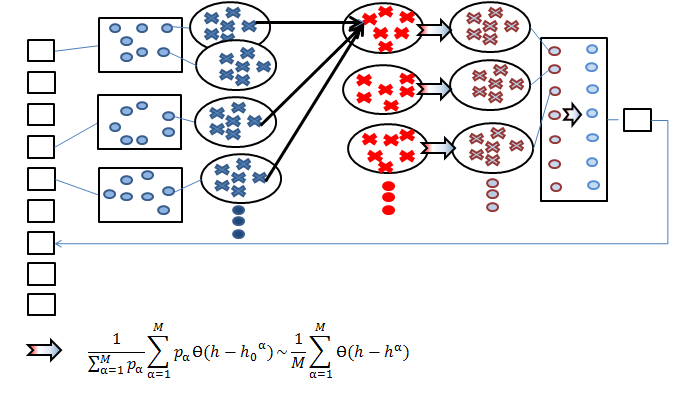
\includegraphics[scale = 0.7]{img/algoimg2.png}
	\caption{A step of the algorithm. In this figure the method used to generate the equilibrium fields is pictured: $K$ sites are chosen randomly. The states are merged according to \ref{merge} (represented with the black lines). Then the state distribution is reweighed in each cluster of the cavity site. Once all reweighs have been done at state level, the clusters are reweighed. The reweighing procedure is represented with the coloured arrow. Once all operations have been done, the new site replaces a site of the system.}
	\label{fig:algoimg}
\end{figure}

\subsection{Observables Evaluation}

Every observable is computed in a similar way to what happened in one step RSB section. There are two main differences from the one step RSB case.

\begin{itemize}

\item{Each observable has to be computed over every state and every cluster}
\item{There are two different derivatives, the $x_s$ derivative, and the $x_C$ one.}

\end{itemize}



\begin{equation}
U= -\sum_{\alpha\gamma} \tanh (\beta v_\alpha\gamma)
\end{equation}

The overlaps are evaluated with the aid of equations \ref{qsite} and \ref{qlink}, this time we have three overlaps, that can be computed in the following way.

\begin{eqnarray}
	q_2 &=& \sum_{\alpha\gamma} \tanh(\beta h^{\alpha\gamma})\tanh(\beta h^{\alpha\gamma}) \nonumber  \\
	q_1 &=&  \sum_{\gamma'\neq\gamma} \tanh(\beta h^{\alpha\gamma'})\tanh(\beta h^{\alpha\gamma})\nonumber \\
    q_0 &=&  \sum_{\alpha'\neq\alpha \gamma'\neq\gamma} \tanh(\beta h^{\alpha'\gamma'})\tanh(\beta h^{\alpha\gamma})\nonumber
\end{eqnarray}

The link overlaps are evaluated with the same set of equations, this time using $v^\alpha$ instead of $h_\alpha$. Again,. we have now to compute three different overlaps

\begin{eqnarray}
	q_2^{(l)} &=& \sum_{\alpha} \tanh(\beta v^{\alpha})\tanh(\beta v^{\alpha})  \nonumber \\
	q_1^{(l)} &=&  \sum_{\gamma'\neq\gamma} \tanh(\beta v^{\alpha\gamma'})\tanh(\beta v^{\alpha\gamma})\nonumber \\
    q_0^{(l)} &=&  \sum_{\alpha'\neq\alpha \gamma'\neq\gamma} \tanh(\beta v^{\alpha'\gamma'})\tanh(\beta v^{\alpha\gamma})\nonumber
\end{eqnarray}

The free energy is obtained summing the site and link contributions (equations \ref{sitedf} and \ref{linkdf}).

\begin{equation}
F = {K+1 \over 2} F_{l} - K F_s
\label{sitepluslink}
\end{equation}

As before, it is also possible to compute the free energy using a different method.

\begin{equation}
F = {K+1 \over 2} F_{iter} - {K-1 \over 2} F_s
\label{saddle}
\end{equation}

The two contributions to the $x_s$-derivative of the free energy are evaluated as in one step RSB case.

\begin{eqnarray}
d_s_{x_s}(x_s,x_C) &=& {-1\over \beta x_s} \log[ \sum_\alpha \exp(-\beta x \Delta {F_s}^\alpha) \log \Delta {F_s}^\alpha ]  \nonumber \\
d_l{x_s}(x_s,x_C)  &=& {-1\over \beta x_s} \log[ \sum_\alpha \exp(-\beta x \Delta {F_l}^\alpha) \log \Delta {F_s}^\alpha ] \nonumber
\end{eqnarray}


\section{The reweighing detail}

The reweighing procedure must generate a population of states distributed in order to satisfy equation \ref{reweighing}.

\begin{equation}
\frac{1}{\sum_\gamma \exp(-\beta x \delta F^{\alpha \gamma}) }\sum_\gamma \exp(-\beta x \delta F^{\alpha \gamma}) \Theta(h-{h_{0}^{\alpha\gamma}}) = \frac{1}{N_s} \sum_\gamma \Theta(h-h^{\alpha\gamma})
\end{equation}

The above equations can be implemented in a computer routine using various methods. In the simpler case we only choose the new states into a set containing the old states,
but with a weight given by their prefactor. In order to extract the new fields with the correct weight, the only operation that must be done is to sum over the weights and find the cumulative function of the distribution, then extract a random number in the unitary interval and check to which state it is associated in the cumulative function of the states.
This is indeed a risky procedure, since every new field is extracted from a discrete set, the one containing the old fields. If the system size is too small the risk is to produce a sample composed of a single field or two. This would make evaluation of every observable obviously go wrong.

I will like to remark that this procedure is done $N_c$ times for each iteration step, and one time reweighing $N_s$ variables, so a low complexity in this phase is mandatory.

\subsection{A more refined reweighing}

In this subsection I would like to spend a few words on the possibility of improving the reweighing procedure used in the algorithm runs. The algorithm just described is very simple to understand conceptually, but unfortunately it suffers a big bias given by the fact that it reweighs choosing the new elements from the starting set of the old ones. This in the large $N$ limit will not be a problem, but if the number of available starting states is small there is a chance that the algorithm will return a series of trivial results in a finite time, having generated for example the same value for all the states after the reweighing. An improvement of the reweighing procedure, however, will risk to overweigh the computational effort of the routine. An important thing to remark is that when one has to reweigh at the state level it is simple to create such routine, but when reweighing at cluster level the operation that one must do are conceptually different.

Let's start with the state level reweigh. In this case we have a set $\mathcal(S)$ of fields that sample a probability distribution. First of all we may sort the elements of $\mathcal(S)$, then we choose an element of $\mathcal(S)$ with a probability distribution given by each weight, let's call it $h_i$, where $i$ indicizes the element after the sorting procedure. Then we extract the new field in the interval that has as extremals $h_{i+1}$ and $h_i-1$. If the site chosen is an extremal, we may use the bounding support $[-K,K]$.

This procedure has the advantage of reshuffling a bit the numerical values of the data. This would make the algorithm stable even with small samples.

When we try to extend this reweigh to the cluster level, we need to slightly modify it. Since the data that we must reweigh now is not a collection of points, but instead a collection of probability distributions, we first need a definition of distance that will be used as a comparator in the sorting procedure. A common choose \cite{kullback} is to use the Kullback Leibler divergence as a metric (though it is not a well defined metric, since it is not symmetric). We recall that the Kullback Leibler divergence between two distributions $P$ and $Q$ measures how much information is lost when $Q$ is used to approximate $P$ and is defined as
\begin{equation}
D(P,Q) = \sum_i \log({P_i \over Q_i})P_i
\end{equation}
An ordering procedure could take Q as a the uniform distribution (we are sorting using the entropy of each distribution now) and sort the element with this criterion. The following step is to generate the new distribution. This can be done in an intuitive way similarly to what has been done for the states.

The last passage is the reshuffling of the new fields in each cluster, and then the reshuffle for each cluster. This is mandatory because the ordering procedure introduces a bias, and the reshuffle sets again the correct situation. The reshuffle procedure is very fast (linear in the data size) and typically the Fisher Yates shuffle is used \cite{shuffle}.

\subsection{The effect of reweighing and the meaning of x}

Let's point out how the reweighing of the fields modifies the field distribution. In this section I would like to a couple of graphs representing how the fields will evolve without reweighing. If we try to evolve the fields set without reweighing (no matter how many states or how many clusters we have) we simply obtain the RS algorithm. 

As we can see using appendix C, a value of $x=0$ means that each weight except one is zero. Thus
only those those states associated with that weight are statistically relevant. Ths is equivalent to an assumption that no RSB is present at that level. As an opposite situation, a value for $x$ equal to one means that each state
has the same proper weight, sending the measure of each state to zero. As we can see, the level two $x$ variable, $x_C$, is not that far from zero. This shows a result anticipated before, two step RSB is present, but its
improvement from the one step solution is more subtle than the one obtained passing from RS to one step RSB. So the effect of the reweighing could be small at low values of $x$. In order to make
the distinction clear to the observer, I ran the algorithm once with a value of $x_C = 1$ and $x_s = 1$. The effect of the reweighing is pictured in figure \ref{reweighfig}.

\begin{figure}
  \centering
  % Requires \usepackage{graphicx}
  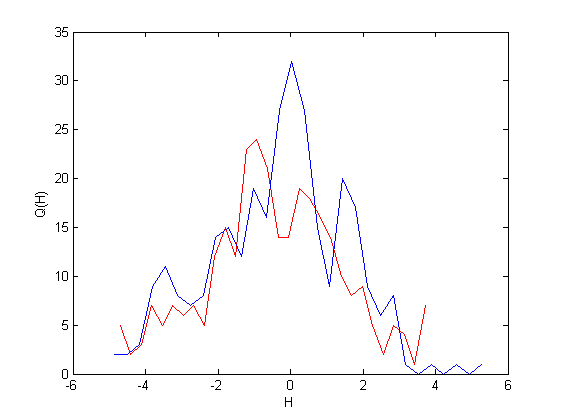
\includegraphics[scale = 0.7]{img/reweigh.pg}
  \caption{Reweighing of the fields $h_0^{\alpha_0 \gamma}$ in cluster $0$ at a state level with $x_C=1,x_s = 1$. In blue we have the fields distribution before the reweighing, in red the distribution after the reweigh.}\label{reweighfig}
\end{figure}






